\documentclass{standalone}
\usepackage{pgfplots}
\pgfplotsset{compat=newest}
\begin{document}
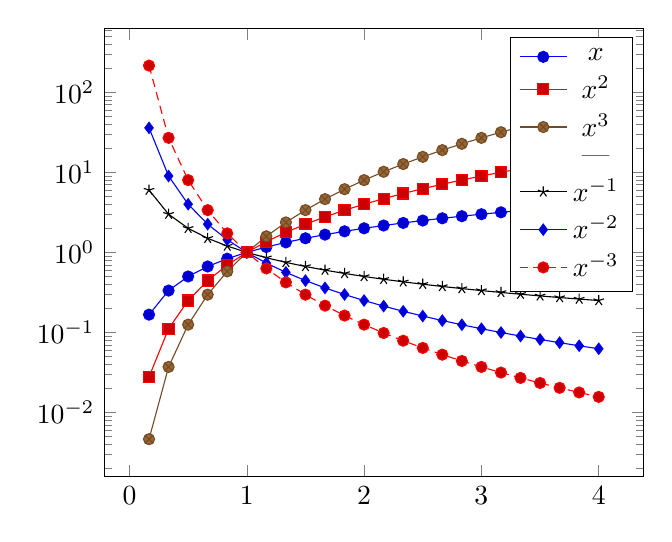
\begin{tikzpicture}
\begin{semilogyaxis}[
	domain=0:4,
]
	\addplot {x};   \addlegendentry{$x$}
	\addplot {x^2}; \addlegendentry{$x^2$}
	\addplot {x^3}; \addlegendentry{$x^3$}
	\addlegendimage{empty legend}
	\addlegendentry{---}
	\addplot {x^(-1)}; \addlegendentry{$x^{-1}$}
	\addplot {x^(-2)}; \addlegendentry{$x^{-2}$}
	\addplot {x^(-3)}; \addlegendentry{$x^{-3}$}
\end{semilogyaxis}
\end{tikzpicture}
\end{document}
